% !TEX encoding = UTF-8
% !TEX TS-program = pdflatex
% !TEX root = ../tesi.tex

%**************************************************************
\chapter{Strumenti e tecnologie utilizzate}
\label{cap:strumenti-tecnologie}

%**************************************************************

\intro{Tale capitolo racchiude gli strumenti utilizzati e le tecnologie impiegate durante la realizzazione del progetto. In particolare verra analizzato il dominio di utilizzo di esse e le varie meotodologie utilizzate.}\\

%**************************************************************
\section{Apache Flink}
\textit{Apache Flink} è un \gls{framework} di \textit{data processing engine} per l'elaborazione e processamento di dati in modo distribuito.
La forza di \textit{Flink} è quella di trattare dati in differenti formati, opportuni per il dominio applicativo più consono per l'utente, infatti i dati possono essere di tipo \gls{stateful} che \gls{stateless} e tali flussi possono essere illimitati (\gls{unbounded streams}) o limitati (\gls{bounded streams}). \textit{Flink} è stato progettato per funzionare in tutti i comuni ambienti \gls{cluster}.

\subsection{DataStream e DataStrem API}
In \textit{Apache Flink} i dati processati in un programma vengono rappresentati dalla classe speciale \textit{DataStream}.
Tali dati possono essere finiti o illimitati, e le \gls{api} utilizzate per lavorare su questi due differenti tipoligie di dati è la stessa, rendendo il tutto trasparente per l'utente programmatore.\\
Carattestiche fondamentali dei \textit{DataStream} sono:
\begin{itemize}
	\item{\textbf{immutabilità:} una volta creati non è possibile aggiungere o rimuovere elementi;}
	\item{\textbf{soggetti a trasformazioni:} non è possibile ispezionare gli elementi al proprio interno, ma solo lavorare su di essi utilizzando le \textit{DataStream \gls{api}}, che vengono definite, appunto, trasformazioni.}
\end{itemize}
La creazione di un \textit{DataStream} necessità di avere una sorgente iniziale (la quale può essere, per esempio, una coda \gls{Apache Kafka}) e da questo si possono derivare numerosi flussi e combinarli utilizzando le \gls{api} esposte, nonchè gli operatori descritti nella sezione \S\ref{sec:operatori}.
Le \textit{DataStream \gls{api}} supportano differenti modalità di esecuzione, le quali permettono di avere un approccio più mirato in base all'utilizzo effettivo dell'utente.\\
Le modalità principali di esecuzione sono:
\begin{itemize}
	\item{\textbf{Esecuzione \textit{streaming}:} tratta principalmente di flussi illimitati (\gls{unbounded streams}) i quali hanno la caratteristica di non terminare mai. I dati vengono processati ininterrottamente, continuando ad aggiornare l'\textit{output} prodotto. In questa modalità le attività esecutive all'interno della \gls{pipeline} del programma continuano ad essere processate in contemporanea, senza stanziarsi in una fase specifica. Questo implica che la \gls{pipeline} non arriverà mai ad uno stadio di terminazione;}
	\item{\textbf{Esecuzione \textit{batch}:} tratta solo flussi limitati (\gls{bounded streams}). Questa procedura permette a \textit{Flink} di ottimizzare l'esecuzione basandosi sul flusso conosciuto, il quale ha un inizio ed una fine. In questa modalità le varie attività all'interno della \gls{pipeline} del programma possono essere eseguite una dopo l'altra, permettendo di passare alla fase successiva solo quando si è terminata quella precedente (quindi non in contemporanea come avviene per l'esecuzione \textit{streaming}). I dati fra una fase ed un'altra vengono salvati in una memoria non temporanea per permettere a \textit{Flink} di ripartire da un determinato \textit{step} senza rieseguire l'intero programma.}
\end{itemize}

\myParagraph{Table API}
\textit{Apache Flink} dispone di due \gls{api} relazionali, l'\textit{\gls{api} Table} e \textit{\gls{sql}}, per un flusso unificato e l'elaborazione \textit{batch}. L'\textit{\gls{api} Table} consente la composizione di \gls{query} da operatori relazionali come selezione, filtro e \textit{join} in modo molto intuitivo. Le \gls{query} specificate in entrambe le interfacce hanno la stessa semantica e specificano lo stesso risultato indipendentemente dal fatto che l'\textit{input} sia continuo (\textit{streaming}) o limitato (\textit{batch}).\\
In particolare l'\textit{\gls{api} Table} è un \textit{super set} del linguaggio \gls{sql} ed è appositamente progettato per lavorare con \textit{Apache Flink}. L'\textit{\gls{api} Table} è un'\gls{api} integrata nel linguaggio per \textit{Scala}, \textit{Java} e \textit{Python}. Invece di specificare le \gls{query} come valori di tipo stringa come nel comune linguaggio \gls{sql}, vengono definite in uno stile integrato nei linguaggi citati precedentemente.

\myParagraph{Query e DataStream}
La tabella sottostante mette a confronto l'algebra relazionale tradizionale e l'elaborazione di un flusso illimitato riguardo i dati in \textit{input}, l'esecuzione e l'\textit{output} finale.

\begin{table}[H]
\caption{Tabella di confronto fra l'algebra relazione e l'elaborazione di un flusso illimitato}
\label{tab:algebraRelazionale-flussoIllimitato}
\begin{tabularx}{\textwidth}{XX}
\hline
\textbf{Algebra relazionale} & \textbf{Flusso illimitato}\\
\hline
Le relazioni (o tabelle) sono (multi)insiemi limitati di tuple.     & Un flusso illimitato è una sequenza infinita di tuple. \\
\hline
Una \gls{query} eseguita su dati \textit{batch} (ad esempio, una tabella in un database relazionale) ha accesso ai dati di \textit{input} completi.    & Una \gls{query} su un flusso illimitato non può accedere a tutti i dati quando viene eseguita e deve aspettare la trasmissione dei dati. \\
\hline
Una \gls{query} eseguita su dati \textit{batch} termina dopo aver prodotto un risultato fissato, cioè non modificabile dopo l'esecuzione. & Una \gls{query} su un flusso illimitato aggiorna continuamente il suo risultato in base ai \textit{record} ricevuti e non viene mai completata. \\
\hline
\end{tabularx}
\end{table}%

Come si evince, i flussi illimitati non lavorano su tabelle statiche, bensì dinamiche. Infatti, le \textit{Dynamic tables} sono il concetto centrale delle \textit{\gls{api} Table} di \textit{Flink} per permettere ad esse di lavorare su un flusso \textit{streaming}.\\
Le tabelle dinamiche cambiano nel tempo e l'interrogazione su di esse produce una \textit{\gls{query} continua}, ed essa produce risultati dinamici, aggiornando continuamente la sua tabella dei risultati (dinamica) per riflettere le modifiche sulle sue tabelle di \textit{input} (dinamiche). È importante notare che un \textit{output} di una \gls{query} continua è sempre semanticamente equivalente al risultato della stessa \gls{query} eseguita in modalità \textit{batch} su uno \gls{snapshot} delle tabelle di \textit{input}.



\subsection{Operatori}\label{sec:operatori}
Gli operatori di \textit{Flink} sono delle procedure per trasformare \textit{DataStream} in altri \textit{DataStream}. Sono utilizzati principalmente per modificare il tipo di flusso di un \textit{DataStream}, il quale appunto verrà filtrato, mappato o combinato con altri flussi per produrre un differente \textit{DataStream}. Nelle sezioni sottostanti verranno descritti i principali operatori utilizzati, i quali non rappresentano la totalità degli operatori disponibili. Per l'elenco completo si rimanda alla documentazione ufficiale di \textit{Apache Flink}.

\myParagraph{FlatMap}
Operatore che dato un elemento, ne produce in \textit{output} uno, zero o molteplici. Tale operatore trasformerà un dato \textit{DataStream} in un altro \textit{DataStream}. La procedura di trasformazione è definita dall'utente e per ogni elemento del \textit{DataStream} verrà applicata tale logica per andare a definire l'\textit{output} atteso. Di seguito la struttura appena descritta.

\begin{minted}{scala}
dataStream.flatMap { str => str.split(" ")}
\end{minted}
	
	
\myParagraph{CoFlatMap}
Operatore che dato un elemento, ne produce in \textit{output} uno, zero o molteplici. Tale operatore trasforma un \textit{ConnectedStream} in un \textit{DataStream}. La differenza con l'operatore \textbf{FlatMap} è che tale operatore lavorerà su due \textit{DataStream} connessi fra di loro, e come per l'operatore nella sezione precedente, verrà prodotto in \textit{output} un unico \textit{DataStream} secondo una logica definita dall'utente. Di seguito la struttura appena descritta.

\begin{minted}{scala}
connectedStreams.flatMap(
    (_ : Int) => true,
    (_ : String) => false
)
\end{minted}

\myParagraph{KeyBy}
Operatore che suddivide un flusso in partizione disgiunte. Tale operatore trasforma un \textit{DataStream} in un \textit{KeyedStream} trattando gli elementi che hanno chiave uguale nella stessa partizione. Internamente, \textit{KeyBy} è implementato con il partizionamento \textit{hash}.
La chiave deve essere intesa come univoca.
Di seguito la struttura appena descritta.
\begin{minted}{scala}
dataStream.keyBy(_.someKey)
dataStream.keyBy(_._1)
\end{minted}

\myParagraph{ProcessFunction}
Operatore di basso livello che da accesso ai blocchi base di uno \textit{Stream}:
\begin{itemize}
	\item{\textbf{eventi:} elementi dello \textit{stream};}
	\item{\textbf{stati:} stati tolleranti agli errori, consistenti e supportati solo nei \textit{KeyedStream}. La \textit{ProcessFunction} da accesso allo stato tramite il \textit{RuntimeContext}, in modo simile a quanto avviene negli altri operatori che hanno accesso allo stato;}
	\item{\textbf{\textit{timer}:} tempo relativo all'evento e tempo relativo al processamento dei dati, anch'esso supportato solo nei \textit{KeyedStream}. Per una descrizione più approfondite del \textit{timer} fare riferimento alla sezione \S\textbf{Timer} sottostante.}
\end{itemize}

Per creare una \textit{ProcessFunction}, serve implementare il metodo astratto \textit{processElement}, nella quale va implementata la logica di gestione degli elementi. Inoltre, per usufruire dello \textbf{stato} e del \textbf{\textit{timer}}, come descritto precedentemente, bisogna basarsi su un \textit{KeyedStream}. Di seguito è stato deciso di analizzare due principali operatori derivati dalla \textit{ProcessFunction}, quali \textbf{KeyedProcessFunction} e \textbf{KeyedBroadcastProcessFunction}, ampiamente utilizzati durante il periodo di stage.

\myParagraph{KeyedProcessFunction}
La \textit{KeyedProcessFunction} è un'estensione di \textit{ProcessFunction}, la quale permette l'accesso alla chiave dei \textit{timer} nel suo metodo \textbf{\textit{onTimer}}. Di seguito un esempio relativo all'estensione della classe \textit{KeyedProcessFunction}, dove all'interno del metodo \textit{onTimer} avviene l'accesso alla chiave dei timer. I parametri \textbf{K}, \textbf{I} e \textbf{O} indicano rispettivamente il \textbf{tipo della chiave}, il \textbf{tipo dell'elemento in \textit{input}} e il \textbf{tipo dell'elemento in \textit{output}}.

\begin{minted}{scala}
class Example extends KeyedProcessFunction[K, I, O] {

  override def processElement(
      value: I, 
      ctx: KeyedProcessFunction[K, I, O]#Context, 
      out: Collector[O]): Unit = {
      
      	// ...
  }

  override def onTimer(
      timestamp: Long, 
      ctx: KeyedProcessFunction[K, I, O]#OnTimerContext, 
      out: Collector[O]): Unit = {
      
      	var key = ctx.getCurrentKey
      
      	// ...
  }
}
\end{minted}
\myParagraph{KeyedBroadcastProcessFunction}
La \textit{KeyedBroadcastProcessFunction} è un'estensione di \textit{ProcessFunction}, la quale permette l'elaborazione di due flussi entranti, quello \textit{broadcast} e quello non \textit{broadcast}. Il punto chiave di questo operatore è che il \textbf{\textit{Broadcast State}}, il quale viene gestito dal flusso \textit{broadcast}, è condiviso fra tutte le istanze parallele dell'operatore, quindi ogni calcolo effettuato in questo flusso garantirà una modifica allo stato di esso che si rifletterà in ogni istanza dell'operatore, a differenza del lato non \textit{broadcast}. Di seguito un esempio relativo all'estensione della classe \textit{KeyedBroadcastProcessFunction}, dove i parametri \textbf{K}, \textbf{I1}, \textbf{I2} e \textbf{O} indicano rispettivamente il \textbf{tipo della chiave}, il \textbf{tipo dell'elemento in \textit{input} nel flusso non \textit{broadcast}}, il \textbf{tipo dell'elemento in \textit{input} nel flusso \textit{broadcast}} e il \textbf{tipo dell'elemento in \textit{output}}.
\begin{minted}{scala}
class Example extends KeyedBroadcastProcessFunction[K, I1, I2, O] {

  override def processElement(
      value: I1, 
      ctx: KeyedBroadcastProcessFunction[K, I1, I2, O]#ReadOnlyContext, 
      out: Collector[O]): Unit = {
      
      	// ...
  }
  
  override def processBroadcastElement(
      value: I2, 
      ctx: KeyedBroadcastProcessFunction[K, I1, I2, O]#Context, 
      out: Collector[O]): Unit = {
      
      	// ...
  }
}
\end{minted}

\myParagraph{Timer}\label{sec:timer}
Tutti e due i tipi di \textit{timer} (tempo relativo all'evento e tempo relativo processamento di tale) sono gestiti dal \textit{TimeService}. Ogni volta che viene chiamato l'operato \textit{ProcessElement} viene fornito un oggetto chiamato \textit{Context} il quale da accesso al \gls{timestamp} relativo all'evento e ad un oggetto chiamato \textit{TimeService}, il quale permette di registrare il \textit{timer} per permettere future elaborazioni. Per ogni coppia \textit{chiave}-\gls{timestamp} esiste un solo \textit{timer}, se più \textit{timer} sono settati per lo stesso \gls{timestamp}, solo uno verrà richiamato. \textit{Flink} sincronizza internamente l'invocazione della funzione \textit{processElement} e \textit{onTimer}, rendendo tale sincronizzazione trasparente per l'utente. I \textit{timer} sono tolleranti verso gli errori, infatti \textit{Flink} salva tale \textit{timer} tramite il meccanismo di \textit{checkpoint} (\S\ref{sec:checkpoint}) come avviene per gli stati.


\subsection{Scalabilità}
\textit{Flink} è progettato per eseguire applicazioni di \textit{streaming} \gls{stateful} su qualsiasi scala. Le applicazioni vengono parallelizzate in migliaia di attività che vengono distribuite ed eseguite contemporaneamente in un \gls{cluster}. Pertanto, un'applicazione può sfruttare quantità virtualmente illimitate di CPU, memoria principale, disco e \textit{Input-Output} di rete. Inoltre, \textit{Flink} riesce a gestire quantità elevate di stati all'interno dell'applicazione e grazie al suo algoritmo di \textit{checkpoint} asincrono e incrementale assicura un impatto minimo sulle latenze di elaborazione, garantendo al tempo stesso il processamento dello stato esattamente una ed una sola volta.

\subsection{Alta disponibilità e recovery}
Durante l'elaborazione dei dati in \textit{Apache Flink} può essere necessario memorizzare le informazioni ricevute ad un dato istante dell'elaborazione, come per esempio quando si addestra un modello di \gls{Apprendimento automatico} su un flusso di punti dati, oppure quando è necessario gestire i dati storici. Per fare ciò \textit{Flink} utilizza il meccanismo di salvataggio delle informazioni in \textbf{stati}.\\
Per gestire tale meccanismo, in \textit{Flink} vengono sfruttate le chiavi passate durante l'elaborazione di un flusso. Lo stato relativo alla chiave viene mantenuto in quello che può essere considerato un archivio chiave/valore incorporato. Pertanto, l'accesso allo stato chiave/valore è possibile \textbf{solo su flussi con chiave}. L'allineamento delle chiavi dei flussi e dello stato assicura che tutti gli aggiornamenti su di esso siano operazioni locali, garantendo la coerenza senza sovraccarico delle transazioni. Questo allineamento consente inoltre a \textit{Flink} di ridistribuire lo stato e regolare il partizionamento del flusso in modo trasparente per l'utente programmatore.

\begin{figure}[H] 
    \centering 
    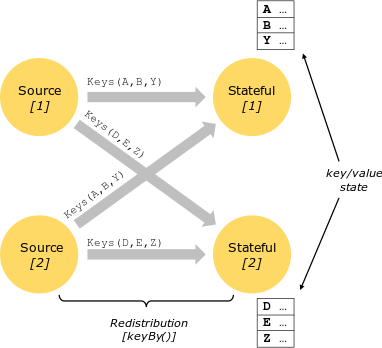
\includegraphics[width=0.5\columnwidth]{tecnologieUtilizzate/flink/state_partitioning.png} 
    \caption{Parallelizzazione del processamento del flusso per chiave in \textit{Apache Flink}}
\end{figure}

\myParagraph{Checkpoint}\label{sec:checkpoint}
Durante l'elaborazione dei dati possono avvenire degli errori che non permettono la continuità del processamento dei dati. \textit{Flink} permette di essere tollerante a questi errori tramite il meccanismo di \textbf{\textit{checkpoint}}. Un \textit{checkpoint} contrassegna un punto specifico in ciascuno dei flussi di \textit{input} insieme allo stato corrispondente per ciascuno degli operatori. Un flusso di dati in \textit{streaming} può essere ripreso da un \textit{checkpoint} mantenendo la coerenza (cioè elaborando il dato esattamente una volta) ripristinando lo stato degli operatori e riproducendo i \textit{record} dal punto prefissato dal \textit{checkpoint}.\\
Durante il processamento, in caso di errori (come errori di rete), \textit{Flink} interrompe il flusso di dati in \textit{streaming} ed esegue le seguenti operazioni:
\begin{itemize}
	\item{Il sistema riavvia gli operatori e li reimposta sull'ultimo \textit{checkpoint} riuscito;}
	\item{I flussi di \textit{input} vengono reimpostati al dato \gls{snapshot} dello stato.}
\end{itemize}
Inoltre viene garantito che tutti i \textit{record} elaborati come parte del flusso di dati parallelo riavviato non abbiano influito sullo stato del \textit{checkpoint} precedente.
Il meccanismo di \textit{checkpoint} (sia a livello di creazione che di ripristino da esso), se configurato durante l'elaborazione, è totalmente gestito da \textit{Flink}, rendendolo trasparente per l'utente.

\myParagraph{Savepoint}
Tutti i programmi che utilizzano il \textit{checkpoint} possono riprendere l'esecuzione da un \textbf{\textit{savepoint}}. I \textit{savepoint} consentono di aggiornare sia i programmi (quindi la logica al loro interno), che il \gls{cluster} di \textit{Flink}.\\
I \textit{savepoint} si possono considerare come dei veri e propri \textit{checkpoint}, che acquisiscono uno \gls{snapshot} del programma e lo scrivono in un \textit{back-end} di stato. I \textit{savepoint} si affidano al normale meccanismo di \textit{checkpoint}, descritto nella sezione \S\ref{sec:checkpoint}, per fare ciò. La differenza sostanziale con un \textit{checkpoint} è che il \textit{savepoint}:
\begin{itemize}
	\item{viene creato manualmente dall'utente;}
	\item{non viene eliminato quando viene eseguito un \textit{checkpoint} in un dato istante successivo al \textit{savepoint}.}
\end{itemize}


\subsection{Serializzazione}
Per salvare e ripristinare i dati durante la creazione di un \textit{checkpoint} o \textit{savepoint}, \textit{Flink} serializza e deserializza i dati in formato binario. Questo rende comprensibile il formato dei dati in qualunque sistema di gestione di essi.\\
\textit{Flink} pone alcune restrizioni sul tipo di elementi che possono trovarsi in un \textit{DataSet} o \textit{DataStream}. La ragione di ciò è che il sistema analizza i tipi per determinare strategie di esecuzione più efficienti.\\
La \gls{serializzazione} predefinita di \textit{Apache Flink} può essere suddivisa approssimativamente nei seguenti gruppi:

\begin{itemize}
	\item{
Serializzatori speciali forniti da \textit{Flink} per i tipi base (primitive \textit{Java} e loro forma \textit{boxed}), \textit{array}, tipi compositi (\textit{tuple}, \textit{case class} di \textit{Scala}, \textit{Rows}) e alcuni tipi ausiliari (\textit{Option}, \textit{Either}, \textit{Lists}, \textit{Maps}, …);}
	\item{\gls{pojo}, cioè un tipo di classe che soddisfa i seguenti requisiti:
\begin{itemize}
	\item{la classe deve essere pubblica;}
	\item{deve avere un costruttore pubblico senza argomenti (costruttore predefinito);}
	\item{tutti i campi sono pubblici o devono essere accessibili tramite le funzioni \textit{getter} e \textit{setter};}
	\item{il tipo di un campo deve essere supportato da un serializzatore registrato.}
\end{itemize}}
	\item{Tipi generici, cioè tipi di dati definiti dall'utente che non sono riconosciuti come \gls{pojo} e quindi serializzati tramite \textit{Kryo} (\S\ref{sec:kryo}).}
\end{itemize}
In alternativa alla \gls{serializzazione} offerta internamente da \textit{Flink}, si possono creare anche dei serializzatori personalizzati definiti dall'utente, i quali possono integrare altri sistemi di \gls{serializzazione} come per esempio \textbf{\textit{Avro}} (\S\ref{sec:avro}). I serializzatori personalizzati sono molto importanti per quanto riguarda lo \textbf{\textit{State Schema Evolution}}, infatti le applicazioni \textit{streaming} di \textit{Apache Flink} sono generalmente progettate per funzionare a tempo indeterminato o per lunghi periodi di tempo. Come per tutti i servizi di lunga durata, le applicazioni devono essere aggiornate per adattarsi alle mutevoli esigenze. Questo vale anche per gli schemi di dati su cui lavorano le applicazioni, i quali si evolvono insieme all'applicazione stessa.\\
Di seguito vengono analizzati i due \gls{framework} di \gls{serializzazione} citati precedentemente.

\myParagraph{Kryo}\label{sec:kryo}
\textit{Flink} utilizza il \gls{framework} \textit{Kryo} in modo totalmente trasparente per l'utente programmatore sui tipi di dati non riconosciuti come \gls{pojo} o che non sono corredati da serializzatori speciali. Se si utilizza \textit{Kryo}, è importante registrare il tipo di classe per permettere a \textit{Kryo} di memorizzare tale classe in modo che, durante la \gls{serializzazione}, \textit{Kryo} non debba aggiungere i nomi di classe completi come prefisso nel modulo serializzato. \textit{Kryo} usa questo meccanismo di \textit{tag} (interi) per identificare le classi sottostanti e ridurre il sovraccarico della \gls{serializzazione}.



\myParagraph{Avro}\label{sec:avro}
\textit{Flink} offre supporto per il \gls{framework} di \gls{serializzazione} \textit{Apache Avro} tramite la dipendenza \textit{org.apache.flink:flink-avro}. L'\textit{AvroSerializer} di \textit{Flink} può quindi sfruttare le prestazioni e la flessibilità di \textit{Avro}, soprattutto in termini di evoluzione dello schema quando le classi cambiano nel tempo.

\subsection{Testing}\label{sec:flink-testing}
\textit{Flink} espone delle funzionalità interne per permettere la stesura di \textbf{test di unità} relativi ad operatori \gls{stateful} o che utilizzano \textit{timer} e operatori \gls{stateless}. \textit{Apache Flink} offre, inoltre, la funzionalità di \textit{testing} relativa ad un intero \gls{cluster}. Per semplicità, all'interno di questa sezione viene esplicitata la procedura di creazione di un test di unità relativo ad un operatore \gls{stateful}, nonché l'unico tipo di test utilizzato durante il progetto.\\
Il \textit{testing} della funzionalità di un operatore che fa uso di uno stato o di un \textit{timer} implica testare l'interazione tra il codice prodotto dallo sviluppatore e il \textit{runtime} di \textit{Flink}. Per semplificare ciò \textit{Apache Flink} fornisce una raccolta di cosiddetti \textit{test harnesses}, i quali permettono di testare differenti operatori del tipo:
\begin{itemize}
	\item{\textbf{\textit{OneInputStreamOperatorTestHarness}:} per operatori di tipo \textit{DataStreams};}
	\item{\textbf{\textit{KeyedOneInputStreamOperatorTestHarness}:} per operatori di tipo \textit{KeyedStreams};}
	\item{\textbf{\textit{TwoInputStreamOperatorTestHarness}:} per operatori di tipo \textit{ConnectedStreams} di due \textit{DataStreams};}
	\item{\textbf{\textit{KeyedTwoInputStreamOperatorTestHarness}:} per operatori di tipo \textit{ConnectedStreams} di due \textit{KeyedStreams}.}
\end{itemize}

Il funzionamento dei \textit{test harnesses} prevede l'inserimento di \textit{record} nei differenti flussi trattati dall'operatore, il processamento di \textit{watermark} e il controllo riguardo al tempo di esecuzione (\textit{timer}) dell'operatore stesso. Inoltre è possibile fare asserzioni sugli stati interni e sull'\textit{output} dell'operatore, inclusi i \textit{side outputs}. 



%**************************************************************
\section{Scala}\label{sec:scala}
Il linguaggio di programmazione utilizzato all'interno del \gls{framework} \textit{Flink} è \textbf{Scala}. \textit{Scala} (da \textit{Scalable Language}) è un linguaggio di programmazione multi-paradigma studiato per integrare le caratteristiche e funzionalità dei \textbf{linguaggi orientati agli oggetti} e dei \textbf{linguaggi funzionali}. La compilazione di codice sorgente \textit{Scala} produce \textit{Java bytecode} per l'esecuzione su una \gls{jvm}. L'esecuzione di un programma prodotto in linguaggio \textit{Scala} avviene tramite \gls{jre}, il quale semplifica l'integrazione con le applicazioni e le componenti \textit{Java}.\\
Una delle peculiarità più importanti di \textit{Scala}, come accennato in precedenza, è l'integrazione di due paradigmi di programmazione molto noti:
\begin{itemize}
	\item{\textbf{Orientamento agli oggetti:} ogni elemento del linguaggio è un oggetto, inclusi numeri e funzioni che, così, possono essere memorizzate in variabili, essere passate come parametri, rappresentare il risultato di una chiamata di metodo, oppure essere estese tramite ereditarietà;}
	\item{\textbf{Funzionale:} ogni funzione è un valore. \textit{Scala} fornisce un linguaggio molto diretto per definire funzioni anonime (dichiarate e usate senza essere legate ad un nome), supporta funzioni di ordine superiore, permette alle funzioni di essere annidate e supporta funzioni parziali.}
\end{itemize}
Di seguito vengono elencate alcune strutture logiche specifiche di \textit{Scala} considerate importanti e differenti rispetto ai linguaggi di programmazione più conosciuti:
\begin{itemize}
	\item{\textbf{Case class:} le \textit{case class} vengono utilizzate principalmente per la modellazione di dati immutabili. A differenza delle \textit{class}, per istanziare una \textit{case class} non è necessaria la parola \textit{new} e le funzioni \textit{getter} sono automaticamente definite per i parametri del costruttore. Inoltre la comparazione fra \textit{case class} avviene per valori e non per riferimenti, cioè oggetti diversi ma con valori uguali sono considerati eguali;}
	\item{\textbf{Option:} come si evince dal nome, le \textit{Option} di \textit{Scala} sono utilizzate per rappresentare un tipo opzionale, cioè che contiene un valore del tipo specificato oppure no. Se un valore è presente, l'istanza dell'\textit{Option} sarà di tipo \textit{Some(x)}, dove \textit{x} rappresenta il valore del tipo specificato dall'\textit{Option} stessa. Se, invece, il valore non è presente, l'istanza rappresenterà un tipo \textit{None}.}
\end{itemize}
Un'altra caratteristica fondamentale di \textit{Scala} è quella di permettere l'utilizzo dell'astrazione dei tipi. Questo significa che l'utente non è tenuto a specificare nel codice il tipo dei parametri rappresentati, ma vengono dedotti dal contesto tramite il compilatore.


%**************************************************************

\section{ScalaTest}\label{sec:scala-test}
\textit{ScalaTest} è un \gls{framework} per la creazione di test basati sul linguaggio \textit{Scala} o \textit{Java}. \textit{ScalaTest} supporta diversi stili di test, ciascuno progettato per soddisfare un particolare insieme di esigenze. Di seguito viene rappresentato un esempio dello stile \textit{FlatSpec}, stile che è stato utilizzato per la redazione dei test di unità all'interno del progetto:

\begin{minted}{scala}
class SetSpec extends AnyFlatSpec {

  "An empty Set" should "have size 0" in {
    assert(Set.empty.size == 0)
  }

  it should "produce NoSuchElementException when head is invoked" in {
    assertThrows[NoSuchElementException] {
      Set.empty.head
    }
  }
}
\end{minted}

Nello stile \textit{FlatSpec} i nome dei test devono essere scritti secondo la convenzione: "\textit{X should Y}" e/o "\textit{A must B}".\\
Inoltre \textit{ScalaTest} offre i principali costrutti per la progettazione di test come per esempio \textit{Before} e \textit{After}, dove rispettivamente al loro interno viene  prodotto il codice che verrà eseguito prima e dopo di ogni test.



%**************************************************************
\section{Amazon Kinesis}



%**************************************************************
\section{IntelliJ IDEA}
\textit{IntelliJ IDEA} è un ambiente di sviluppo integrato (\gls{ide}) utilizzato prevalentemente per il linguaggio di programmazione \textit{Java}. Sviluppato da \textit{JetBrains} (prima conosciuto come \textit{IntelliJ}), è disponibile sia in licenza \textit{Apache} che in edizione proprietaria commerciale.\\
\textit{IntelliJ IDEA} offre numerose \textit{features} per facilitare lo sviluppo applicativo:
\begin{itemize}
	\item{\textbf{Codifica assistita:} l'\gls{ide} offre il completamento assistito del codice tramite l'analisi del contesto, la navigazione interna del codice che permette di passare da una classe o una parte di codice ad un'altra e il \textit{refactor} del codice stesso;}
	\item{\textbf{Integrazione di \textit{tools} esterni}: viene offerto l'integrazione con numerosi strumenti esterni come quelli relativi al \textit{build/packaging} e quelli relativi al versionamento del codice. In particolare durante la realizzazione del progetto è stato utilizzato il \textit{tool} \textbf{SBT} come strumento di \textit{build/packaging} e \textbf{GIT} come versionatore del codice;}
	\item{\textbf{Supporto a numerosi linguaggi di programmazione}: in particolare per la realizzazione del progetto è stato utilizzato un \textit{plugin} offerto da \textit{IntelliJ IDEA} per la codifica tramite il linguaggio \textbf{Scala} (\S\ref{sec:scala}).}
\end{itemize}

